\documentclass{standalone}
\usepackage{hsbcommon}
%% Show/hide steps for standalone work — edit this line:
\makeatletter\AtBeginDocument{\@buildstepset{1,2}}\makeatother
\begin{document}
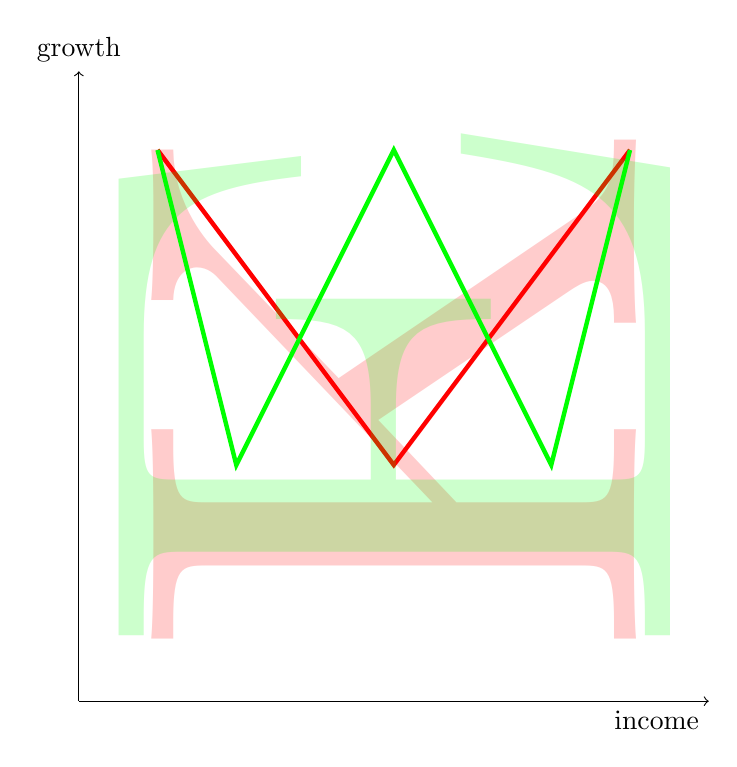
\begin{tikzpicture}
    \tikzset{
        letter/.style={font=\rmfamily}
    }
    %% axis
    \draw[->] (0,0) node[below] {\phantom{x}} -- (8,0) node[below left] {income};
    \draw[->] (0,0) node[left] {\phantom{x}} -- (0,8) node[above] {growth};

    \ifstep{1}{
    \begin{scope}[red]
        \node[letter,rotate=90,opacity=0.2] at (4,4) {
            \resizebox{7cm}{!}{K}
        };
        \draw[ultra thick] (1,7) -- (4,3) -- (7,7);
    \end{scope}
    }

    \ifstep{2}{
    \begin{scope}[green]
        \node[letter,rotate=90,opacity=0.2] at (4,4) {
            \resizebox{7cm}{!}{E}
        };
        \draw[ultra thick] (1,7) -- (2,3) -- (4,7) -- (6,3) -- (7,7);
    \end{scope}
    }
    
\end{tikzpicture}

\end{document}